\chapter[Introduction]{Introduction\label{ch:1_Introduction}}

\section{The magic of superconductors and semiconductors}

Much of condensed matter physics is concerned with understanding and controlling the behavior of electrons on the quantum\hyp{}mechanical level. 
To this end, superconductors and semiconductors are two of the most well\hyp{}studied classes of materials.
Individually, superconductors and semiconductors possess incredible properties with far\hyp{}reaching applications. 
In superconductors, pairing between electrons results in the flow of dissipation\hyp{}less current, even in the presence of disorder.  
The defining characteristic of semiconductors, on the other hand, is a low density of charge carriers.
The chemical potential can thus be controlled directly by applying an electric field (the field effect).  
In some semiconductors, relativistic effects result in enhanced $g$\hyp{}factors and strong spin\hyp{}orbit coupling.

In the context of quantum information processing, the properties of superconductors and semiconductors lend themselves to quantum mechanical control of electrons on vastly different scales. 
In superconducting circuits, a condensate composed of trillions of electrons can behave as a single continuous degree of freedom. 
For instance, the complete quantum mechanical state of a superconducting LC oscillator can be described by the amount of charge on the capacitor.
In contrast, semiconductors lend themselves to control over individual electrons. 
The field effect can be used to trap electrons in quantum dots, while enhanced $g$\hyp{}factors make it easier to achieve a sizeable energy splitting between the spin states. 
In addition, spin\hyp{}orbit coupling can be used to achieve spin manipulation via an AC electric field. 

What would happen if we had the properties of both superconductors \textit{and} semiconductors in the same electronic system? 
What new physics would emerge? 
What additional control could we achieve? 
These are the questions posed by experiments on  \textbf{superconductor\hyp{}semiconductor heterostructures}. 
The basic idea with such heterostructures is that if the contact between the two materials can be made good enough, the electrons can move back and forth across the interface unimpeded (their wavefunctions are no longer localized to one material or the other). 
In this way, the electrons can inherit characteristics of both materials, and simultaneously possess all the properties discussed above. 

The work presented in this thesis was all done on a particular mesoscopic heterostructure: a superconductor\hyp{}proximitized semiconductor nanowire. 
However, there is a critical detail: in the middle of the nanowire, there is a spatial gap in the proximitizing superconductor [Fig. \ref{intro_fig}]. 
The nanowire is thus a particular example of a \textbf{weak link}: two superconductors separated linked by a non\hyp{}superconducting (aka ``normal") region.  
In this thesis, we will refer to this nanowire weak link as a \textbf{Josephson nanowire}.

\begin{figure}
    \centering
    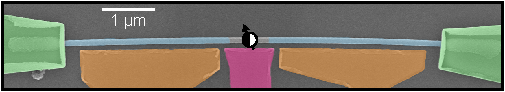
\includegraphics[width = \textwidth]{Chapters/1-intro_fig.pdf}
    \caption[A single spinful quasiparticle trapped in a Josephson nanowire]{\textbf{A single spinful quasiparticle trapped in a Josephson nanowire $\rvert$ }
    Most of the $10~\um$\hyp{}long indium arsenide nanowire is coated in epitaxial aluminum (light blue), but a gap forms a weak link where a single quasiparticle can become trapped.  
    In this thesis, we explore how the spin state of a such a quasiparticle can be detected and manipulated. 
    Gates for electrostatic control are shown in pink/orange, and the leads to the rest of the circuit are shown in green. 
    }
    \label{intro_fig}
\end{figure}

\section{What's so special about a weak link?}

Weak links are the backdrop for what is perhaps the most famous phenomenon in mesoscopic superconductivity: the Josephson effect, in which a dissipation\hyp{}less current flows across the weak link, even in the absence of a voltage bias.
Much less well\hyp{}known than the Josephson effect, however, are the \textbf{Andreev levels}: single-particle, sub-gap, electronic degrees of freedom that are localized to the weak link. 
Fundamentally, it is the Andreev levels that transport the Josephson supercurrent, and it is the Andreev levels that are the focus of this thesis. 

In the context of superconducting qubits, Andreev levels are often forgotten. 
Why is this? 
Typically, superconducting quantum circuits are based on superconductor-insulator-superconductor weak links (also known as tunnel junctions). 
While these weak links possess millions of Andreev levels, the energies of the Andreev levels are very close to (but always below) the superconducting gap. 
As such, they are essentially frozen out, remaining in their supercurrent\hyp{}carrying ground state.
Yet fundamentally, they are fermionic degrees of freedom populated by the electronic spin-1/2 quasiparticle excitations of superconductors.

The physics of the Andreev levels (and therefore emergent Josephson effects) is determined by the geometric and material properties of the host weak link. 
In tunnel junctions, the Andreev level energies remain close to the superconducting gap. 
But as we will see, the Andreev levels of Josephson nanowires can have energies far below the gap edge. 
Moreover, thanks to the properties of the semiconductor, this sub-gap structure is strongly influenced by a rich interplay between superconductivity, electromagnetic field effects, device geometry, and spin-orbit coupling.
In past experiments on Josephson nanowires, these effects have been harnessed to demonstrate gate-tunable weak links for superconducting qubits, non-abelian Andreev levels known as Majorana zero modes, and, critically for this work, spin-split Andreev levels even in the absence of a Zeeman field. 

Can we use the richness of Josephson nanowires to our advantage? 
Can we achieve control over the Andreev levels in ways which were previously impossible? 
What new Andreev physics can we observe?
In this thesis, we explore these questions using the techniques of \textbf{circuit quantum electrodynamics (cQED)}.
Originally developed for manipulation and measurement of superconducting qubits, cQED gives us spectroscopic resolution and time-domain information that is inaccessible in more conventional DC transport experiments. 
Moreover, cQED is less invasive than DC transport. 
While transport necessarily entails pushing electrons through the system under study, in cQED the number of electrons in the circuit is often fixed, and only photons are exchanged with the system. 

\section{Structure of this thesis}

This thesis is arranged into two parts: a main body where we present the ideas and results central to this thesis (chapters 2-5), and a series of later chapters that give detailed explanations and information concerning those same ideas and results. 

In the main chapters, we will first give an overview of how Andreev levels arise in weak links, with a focus on how the Andreev levels of Josephson nanowires differ from those of conventional tunnel junctions. 
We will then discuss how Andreev levels can be probed using cQED, and present as a case study our investigation of pair transitions in Josephson nanowires. 
Finally, we will present the main result of thesis: the realization of the Andreev spin qubit, which is formed from the two spin states of a quasiparticle trapped in the Andreev levels of a Josephson nanowire.  
